%\begin{wrapfigure}{r}{0.30\textwidth}
%  \vspace{-20pt}
%  \begin{center}
%    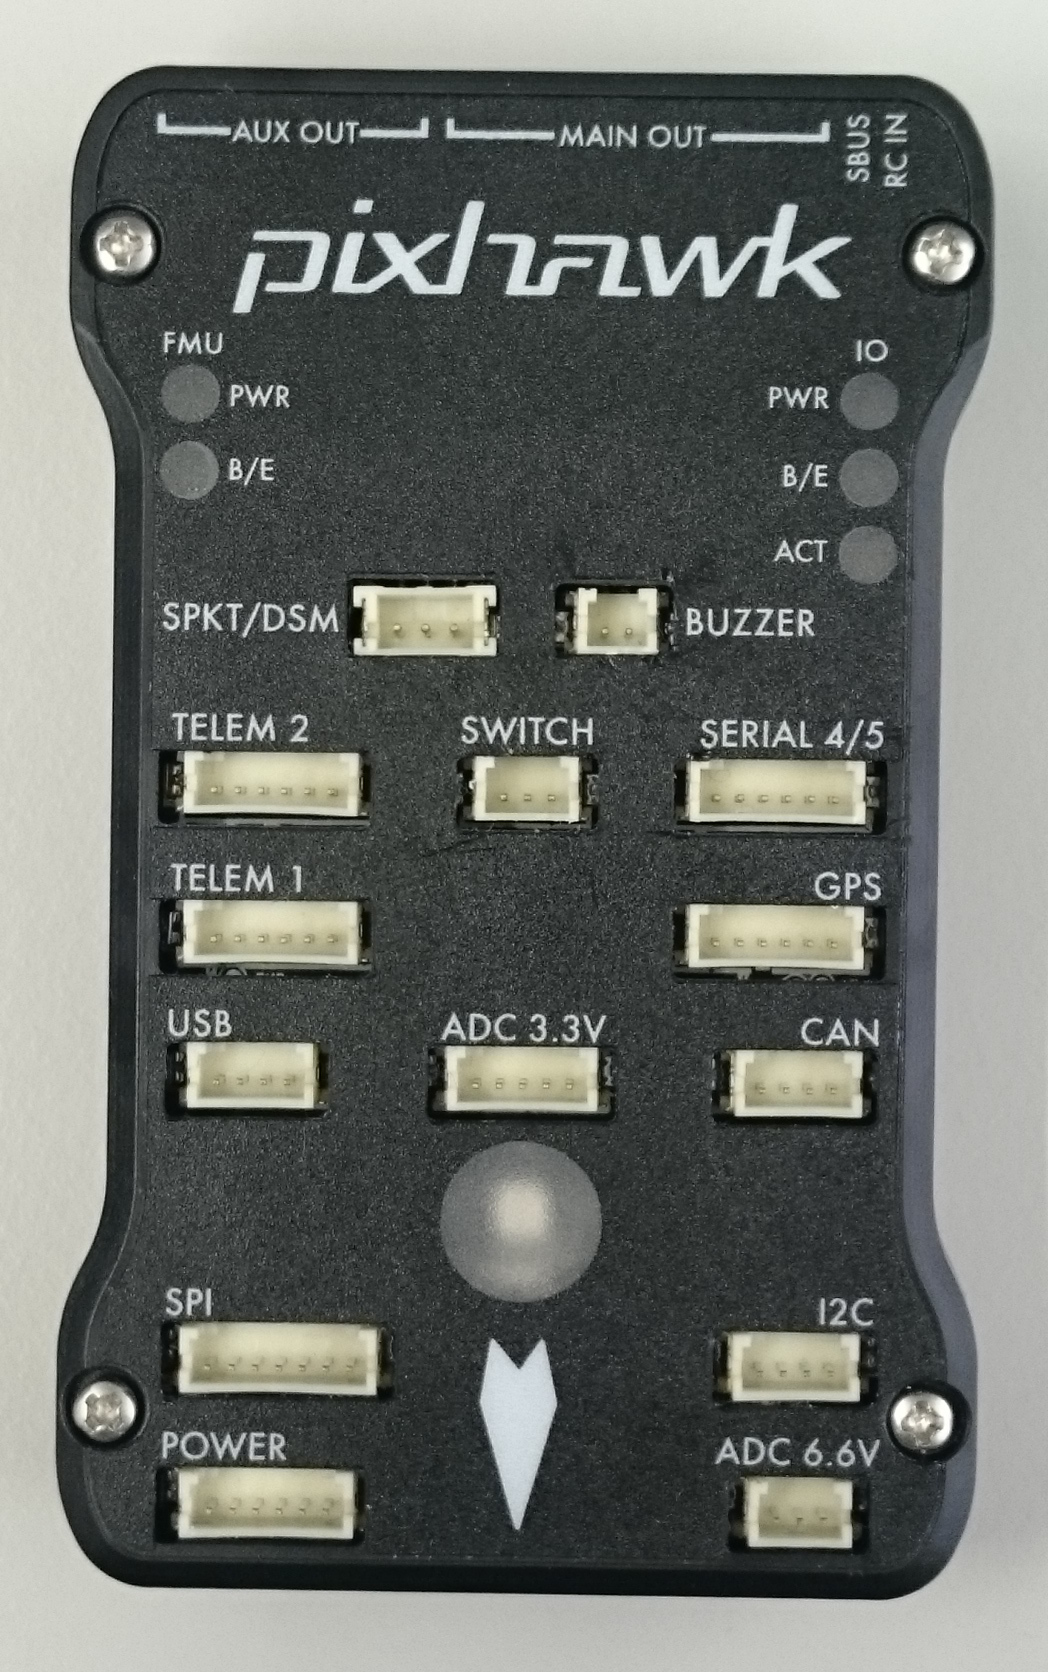
\includegraphics[width=0.28\textwidth]{pic/20_pixhawk/pixhawk_alone.jpg}
%  \end{center}
%  \vspace{-20pt}
%  \caption{Pixhawk}
%  \vspace{-10pt}
%\end{wrapfigure}


Das open-source Projekt Pixhawk ist ein Hochleistungsautopilot für Modellflugzeuge, Multicopter, Helikopter, Autos und Boote. Es wurde an der ETH Zürich entwickelt und ist nun auf dem Markt verfügbar. Das Pixhawk ist die zweite Version des Flugreglers. Für die Verwendung sowie Weiterentwicklung stehen zahlreiche Tools, Anleitungen und eine aktive Community zur Verfügung .\\
Für die Arbeit dient das Pixhawk zur Regelung eines Quadrocopters oder Modellhubschraubers.

\begin{figure}[ht]
  \begin{center}
  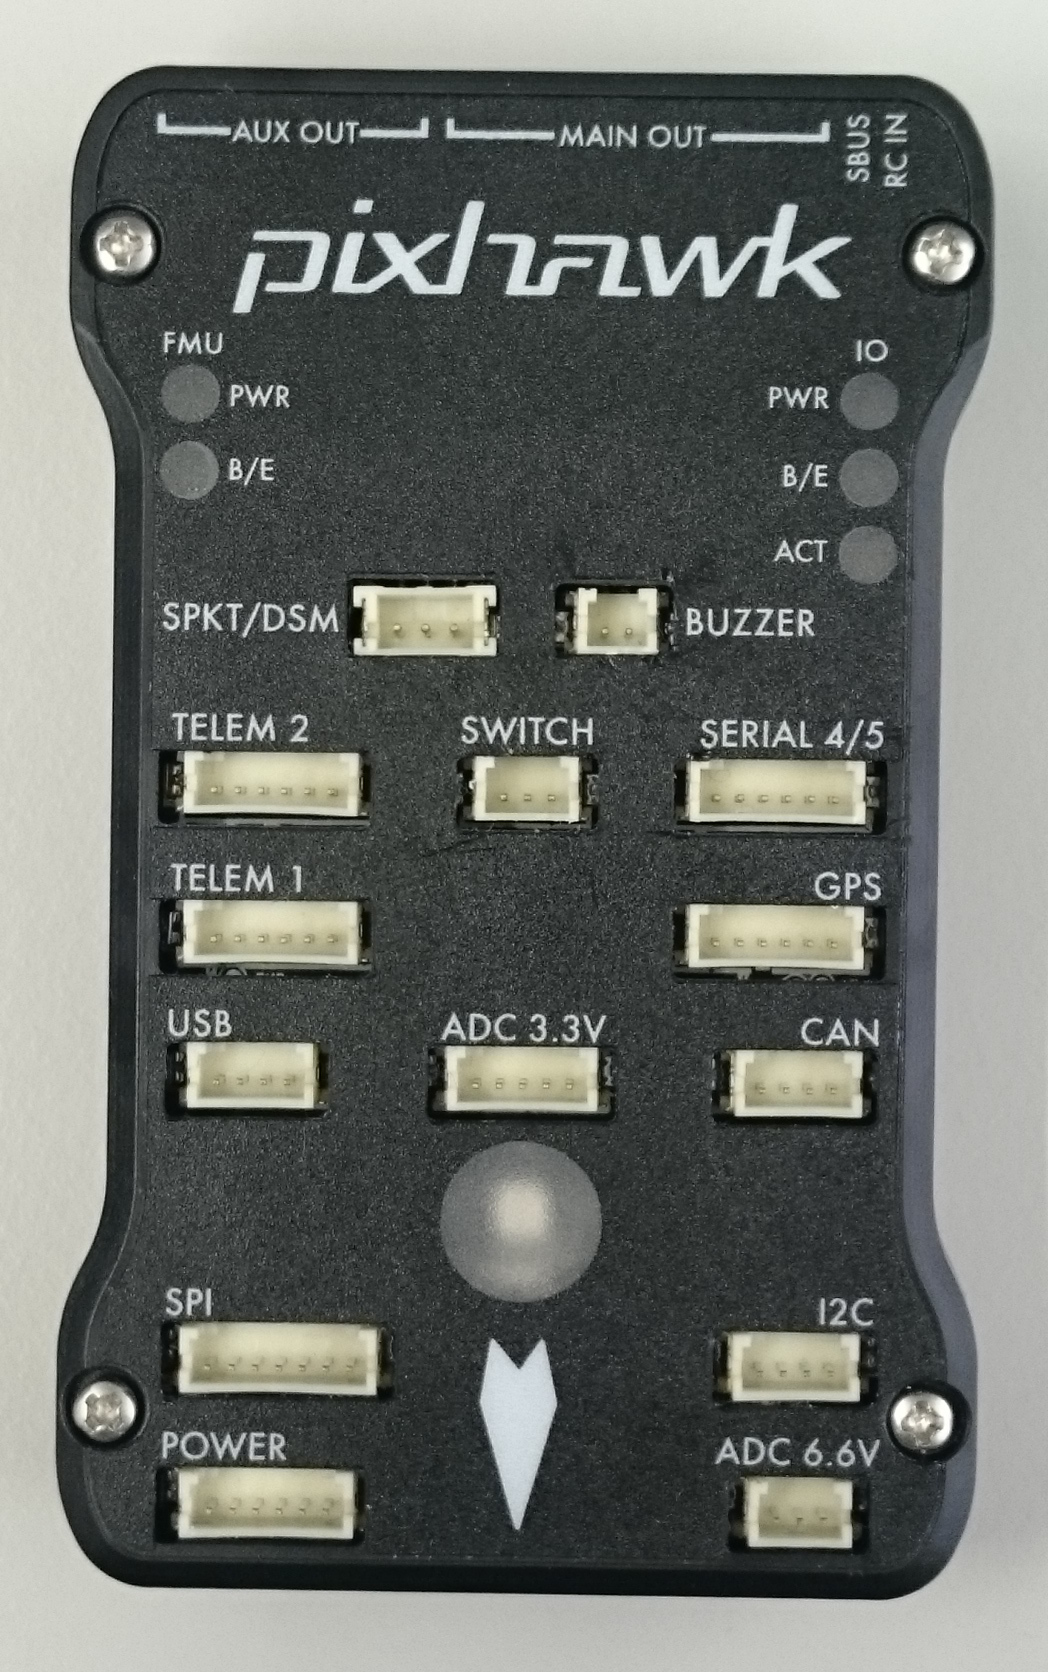
\includegraphics[width=0.3\textwidth]{pic/20_pixhawk/pixhawk_alone.jpg}
  \end{center}
  \caption{Pixhawk}
\end{figure}

Die wichtigsten Features des Pixhawks sind:
\begin{itemize}
\item 32-bit 168 MHz Cortex M4F (floating point unit)
\item 256 KB RAM, 2 MB Flash
\item MPU6000 als Accelerometer und Gyrometer
\item Power Controller mit Ausfallsicherung
\item ESC protection und überstrom Schutz
\item 5x UART, I2C, SPI, CAN, SD Karte, PWM, PPM, AD Wandler
\end{itemize}



\clearpage